\documentclass[twocolumn,oneside,a4paper,12pt]{article}

% ---------------- Para Modificar ---------------- 
\newcommand{\principal}{Volumes}
\newcommand{\conteudo}{}
\newcommand{\turmas}{3~EMSI~A e do 3~EMSI~B}

\date{abril de 2021}

\newcommand{\citacao}{Que nada nos defina. Que nada nos sujeite. Que a liberdade seja a nossa própria substância.}
\newcommand{\autorcitacao}{Simone de Beauvoir}
% ------------------------------------------------

%-------------------------------------------------
\usepackage[english,brazilian]{babel}
\usepackage[alf]{abntex2cite}
\usepackage[utf8]{inputenc}
\usepackage[T1]{fontenc}
\usepackage[top=15mm, bottom=15mm, left=10mm, right=10mm]{geometry}
\usepackage{framed,booktabs,color,hyperref,graphicx}
\usepackage{amsfonts,amsthm,cancel}
\usepackage{subfigure,enumerate,float}
  
\definecolor{shadecolor}{rgb}{0.8,0.8,0.8}
\pagenumbering{arabic}

% Colunas
\usepackage{multicol}
\columnsep=10mm %Espaçamento entre colunas.
\setlength{\columnseprule}{1pt}

% Cabeçalho
\usepackage{fancyhdr}
\pagestyle{fancy}
\lhead{\textbf{\principal}}
\rhead{}
\renewcommand{\headrulewidth}{1pt} % espessura da linha do cabeçalho
\renewcommand{\footrulewidth}{1pt} % espessura da linha do rodapé

% Parágrafo
\setlength{\parindent}{1.25cm}

\newtheorem{problema}{Problema}
\newtheorem{exercicio}{exercicio}
\newtheorem{exemplo}{Exemplo}
\newtheorem{questao}{Questão}

\usepackage[skip=10pt]{caption}
\captionsetup{font={stretch=0.4,small}}

\newcommand{\FRASE}{\textit{``\citacao ''}\\(\textbf{\autorcitacao})}

\title{\LINHAHORIZONTAL \\\textbf{\\ \principal}\footnote{Resumo para os estudos das aulas não presenciais no período de quarentena para as turmas do \turmas .}\\\LINHAHORIZONTAL}

\newcommand{\LINHAHORIZONTAL}{\center \rule{16cm}{1.25pt}}
\newcommand{\sol}{\textbf{Solução}}

\newcommand{\m}[1]{\(\displaystyle {#1}\)}
\newcommand{\M}[1]{\[{#1}\]}

\author{\textbf{Professor Leandro Vieira}\\EREM Regina Pacis\\Palmeirina-PE}
\newcommand{\frase}{\begin{verse} \flushright{\FRASE} \end{verse}}


\begin{document}
\maketitle

\section{Introdução}

No o desenho a seguir esquematiza as ligações, por meio de estradas, entre três cidades: \(A\), \(B\) e \(C\).

	\begin{figure}[!tbh]
	\center
	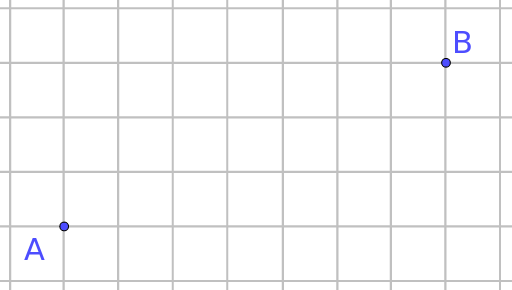
\includegraphics[width=6cm]{00}
	\end{figure}

\begin{enumerate}[(a)]
\item De quantas formas podemos ir de \(A\) até \(C\)?
\item De quantas formas é possível ir de \(A\) até \(C\), e depois de voltar à cidade \(A\) sem repetir caminhos?
\end{enumerate}

\section{O Princípio}
 Se ha \(x\) modos de tomar uma decisão \(D_1\) e, tomada a decisão \(D_1\), há \(y\) modos de tomar a decisão \(D_2\), então o número de modos de tomar sucessivamente as decisões \(D_1\) e \(D_2\) é o produto \(x \cdot y\).
 
\begin{exemplo}
Um rapaz tem 5 camisetas de cores distintas, e 3 bermudas diferentes. De quantas formas ele pode se vestir escolhendo uma camiseta e uma bermuda: 
\end{exemplo}

\begin{exemplo}
A figura a seguir esquematiza a ligação entre três cidades por meio de estradas.

	\begin{figure}[!tbh]
	\center
	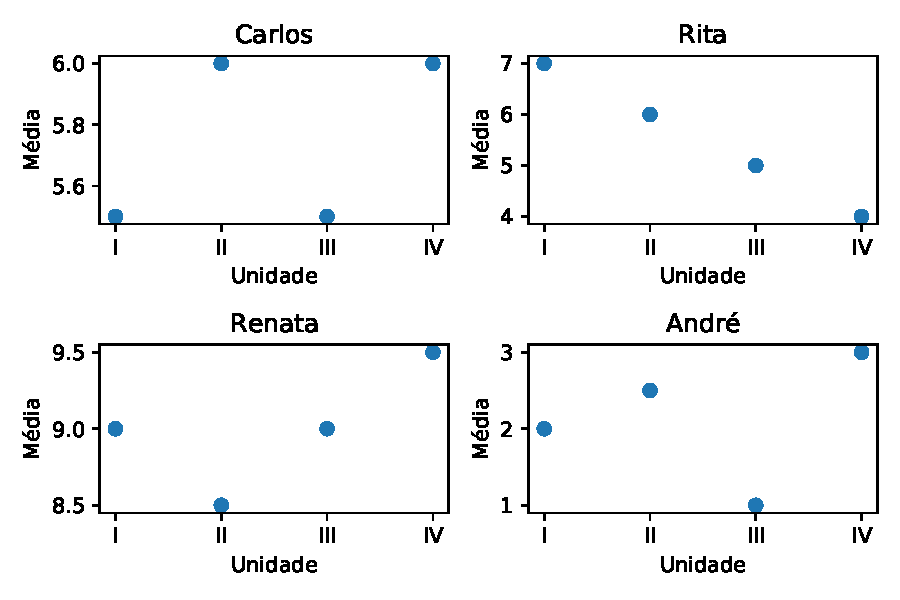
\includegraphics[width=6cm]{01}
	\end{figure}

\noindent As setas pretas representam as estradas asfaltadas, e as setas em vermelho as estradas que não são asfaltadas. Com base nessas informações responda aos seguintes itens:
\end{exemplo}

\begin{enumerate}[(a)]
\item De quantas formas podemos ir de \(A\) até \(C\)?
\item De quantas formas é possível ir de \(A\) até \(C\), e depois voltar à cidade \(A\) sem repetir caminhos?
\item De quantas formas é possível ir de \(A\) até \(C\) passando por uma estrada asfaltada e por uma não asfaltada?
\item Uma competição de motocross passará somente pelas as estradas não asfaltadas entre as cidades \(A\) e \(C\), de quantas formas esse trajeto pode ser feito?
\end{enumerate}

\begin{exemplo}
Na figura a seguir temos a representação de uma bandeira composta por três áreas que devem ser pintadas com um de seis cores disponíveis:
	
	\begin{figure}[!tbh]
	\center
	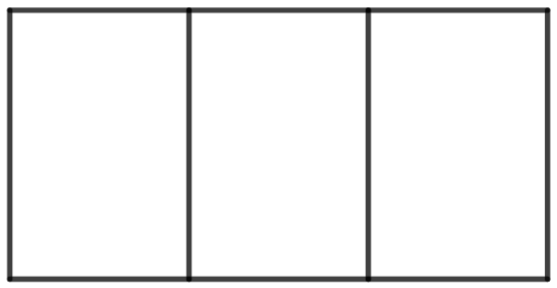
\includegraphics[width=4cm]{02}
	\end{figure}
\end{exemplo}

\begin{enumerate}[(a)]
\item Sem repetir cores, de quantas formas é possível pintar a bandeira?
\item Podendo repetir cores na pintura da bandeira, mas sem que áreas vizinhas tenham a mesma cor, de quantas formas é possível pintá-la?
\end{enumerate}

\begin{exemplo}
Um sistema de senhas de uma empresa aceita senhas feitas com os algarismos 0, 1, 2, 3, 4 e 5. E todas as senhas devem ser compostas por 4 algarismos, sendo que não devem começar por zero. Sabendo que não pode haver repetição de algarismos na senha, qual a quantidades de maneiras diferentes de montar a senha?
\end{exemplo}

\begin{exemplo}
O professor de artes de uma escola também é um apaixonado por matemática. Ele deseja saber de quantas formas é possível colorir a figura, com 8 cores distintas, de forma que setores da figura que tenham arestas em comum não tenham a mesma cor.
	
	\begin{figure}[!tbh]
	\center
	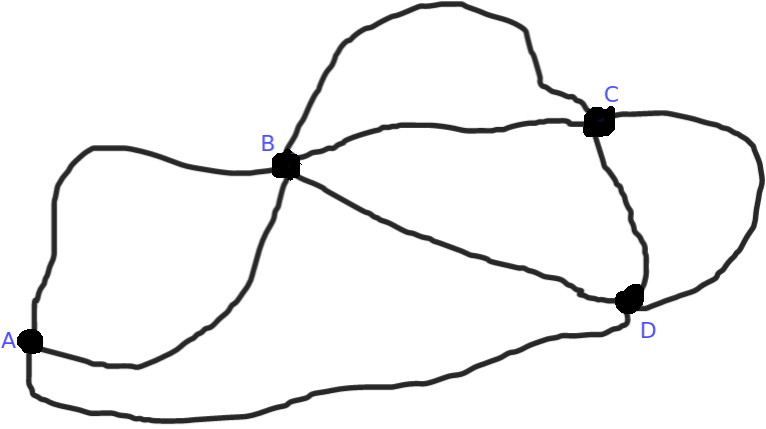
\includegraphics[width=4cm]{03}
	\end{figure}

\noindent De quantas maneiras essa figura pode ser colorida?
\end{exemplo}

\section{Exercicios}

 Página 230: 1, 2, 3, 4

\section{Exemplos de Probabilidade}
\begin{exemplo}
E uma urna estão fichas, cada uma contendo uma das formas de pintar a figura representada a seguir, com uma das cores: azul, verde, rosa e vermelho, de modo que não haja repetição de cores na na pintura das faixas.
	
	\begin{figure}[!tbh]
	\center
	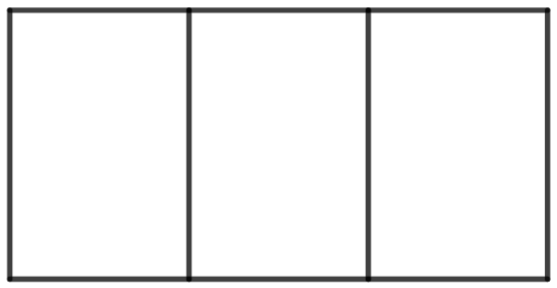
\includegraphics[width=4cm]{02}
	\end{figure}

\noindent Ao tirar uma das fichas, qual a probabilidade de que a mesma tenha uma das faixas pintada de vermelho.
\end{exemplo}


\begin{exemplo}
Em uma urna estão fichas cada uma com um dos números de três dígitos que pode ser formados com os algarismos 0, 1, 2, 3 e 4, retirando-se uma das fichas ao acaso, qual a probabilidade de que o seu número seja par?
\end{exemplo}

\end{document}
